\chapter{Reattori veloci di IV generazione \label{cap1}}
%%%%%%%%%%%%%%%%%%%%%%%%%%%%%%%%%%%%%%%%%%%%%%%%%%%%%%%%%%%%%%%%%%%%%%%%%%%%%%%%
%%%%%%%%%%%%%%%%%%%%%%%%%%%%%

Negli ultimi anni, le sfide associate all'impatto ambientale e ai cambiamenti 
climatici sono diventate più evidenti e di maggiore interesse.
L'energia elettrica prodotta da fonti fossili, che ricopre la maggior parte 
della richiesta di energia mondiale, è causa indiretta dell'innalzamento delle 
temperature medie sul globo terrestre.
Infatti per sua natura, gli impianti termoelettrici che utilizzano il processo 
di combustione di combustibili fossili (carbone, petrolio, gas naturale) per la 
produzione di energia elettrica, liberano in atmosfera notevoli quantità di 
$CO_2$ (anidride carbonica) responsabile dell'aumento dell'effetto serra.

Pertanto la necessità di ridurre le emissioni mondiali, ha indirizzato le 
attenzioni verso la produzione di energia elettrica da altri fonti che siano in 
grado di arginare, almeno in parte, il problema del surriscaldamento globale, 
come per esempio le energie rinnovabili e l'energia nucleare.
In questo contesto, l'energia nucleare è stata considerata capace di avere un 
ruolo a lungo termine per soddisfare la crescente domanda di energia, in quanto 
si tratta di una produzione di energia senza emissioni di $CO_2$.
Tuttora il nucleare ricopre un ruolo importante nel panorama energetico sia 
europeo sia internazionale e si spinge la ricerca in questo ambito verso 
tecnologie affidabili dal punto di vista della sicurezza e sostenibili dal 
punto 
di vista economico. \cite{overview}

\section{Fisica del reattore nucleare}

Il reattore nucleare è la principale componente di un impianto nucleare di 
potenza ed è responsabile della produzione di calore attraverso una reazione a 
catena di fissione nucleare controllata. 
La reazione di fissione avviene quando un neutrone viene assorbito da un 
isotopo 
fissile, come atomi pesanti di uranio $^{233}U$, $^{235}U$ o di plutonio 
$^{239}Pu$, il quale si divide in due o più nuclei a minor peso atomico, denominati 
frammenti di fissione, e liberando un certo numero di neutroni (pronti) e 
neutrini.

Durante la reazione di fissione viene rilasciata una notevole quantità di 
energia, dovuta dalla rottura del legame chimico dell'isotopo fissionato e la 
maggior parte di essa è sotto forma di energia cinetica dei frammenti di 
fissione.
Inoltre i frammenti di fissione sono isotopi instabili e pertanto subiranno un 
processo di decadimento radioattivo che porterà al rilascio di ulteriore energia
e generalmente accompagnato dall'emissione anche di altri neutroni, definiti 
ritardati.
\Figure[scale=0.8]{./graph/fragyield}{Frammenti di 
fissione per i principali isotopi fissili per neutroni a 400keV.}{fragments}

Per esempio dalla fissione di un atomo di $^{235}U$, si libera in media 
un'energia pari a 207MeV, suddivisi come in Tabella 
\ref{energia_di_fissione}.
I neutroni sono emessi secondo uno spettro energetico $\chi(E)$ con un picco in 
corrispondenza delle energie intorno ai 2MeV, come mostrato in Figura 
\ref{spettro_di_fissione}, i quali potranno indurre a loro volta una successiva 
reazione di fissione causando una reazione a catena che si 
autosostiene.
%%%%%%%%%%%%%%%%%%%%%%%%%%%%%%%%%%%%%%%%%%%%%%%%%%%%%%%
\begin{table}[!htb]
\centering
\begin{tabular}{lc}
\toprule
Prodotti di Fissione & Energia [$MeV$] \\
\midrule
Frammenti di fissione & 168 \\
Emissioni Gamma & 7 \\
Neutroni & 5 \\
Neutrini & 12 \\
Decadimenti Beta & 8 \\
Decadimenti Gamma & 7 \\
\bottomrule     
\end{tabular}
\caption{Suddivisione dell'energia liberata dalla fissione di un atomo di 
Uranio 
$^{235}U$.}
\label{energia_di_fissione}           
\end{table}
%%%%%%%%%%%%%%%%%%%%%%%%%%%%%%%%%%%%%%%%%%%%%%%%%%%%%%%%
\begin{figure}[!htb]
\centering
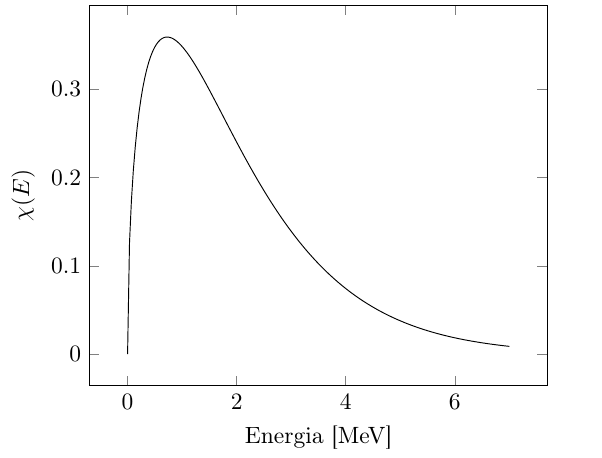
\includegraphics[width=0.7\textwidth]{./figure/reactor/fission_spectrum.png}
\caption{Spettro di emissione di neutroni per fissione per l'uranio $^{235}U$.}\label{spettro_di_fissione}
\end{figure}
%%%%%%%%%%%%%%%%%%%%%%%%%%%%%%%%%%%%%%%%%%%%%%%%%%%%%%%
Uno dei parametri di maggior interesse relativo al concetto di una 
reazione a catena che si autosostiene è definita
dalla costante moltiplicativa effettiva, $k_{eff}$, espressa come 
il rapporto tra la popolazione neutronica presente in una generazione e quella 
della generazione precedente. Inoltre essa rappresenta l'autovalore del 
problema 
del trasporto neutronico in forma stazionaria definito nel Capitolo \ref{cap2}.
Infatti se il $k_{eff}$ risultasse maggiore di 1, la popolazione neutronica 
aumenterebbe esponenzialmente generando così una reazione a catena di fissioni 
incontrollata. Viceversa se fosse minore di 1, la popolazione neutronica 
diminuirebbe pian piano fino a che la reazione a catena si estinguerebbe, 
quindi 
non più autosostenuta, portando così allo spegnimento del reattore stesso. 
Se invece il $k_{eff}$ è uguale a 1 la popolazione neutronica rimanerebbe costante durante l'evoluzione temporale, introducendo il concetto di criticità di un sistema moltiplicante.

Infatti la criticità è strettamente legata al concetto di stazionarietà del 
reattore, 
dove a seguito di una reazione di fissione sono emessi neutroni, i quali possono
causare a loro volta un solo evento di fissione per ottenere una reazione a 
catena controllata e autosostenuta.
Durante un evento di fissione si producono dai 2 ai 3 neutroni e al fine 
di garantire la criticità del sistema, è necessario che uno solo di essi sia in 
grado di sopravvivere e dare luogo a fissione.
Tuttavia potrebbe accadere che il neutrone sia assorbito da un nucleo non di 
combustibile 
oppure semplicemente urtare perdendo o acquistando energia, oppure anche 
incorrere a cattura radiativa senza che esso induca a fissione l'atomo fissile.

La costante moltiplicativa effettiva è valutata attraverso la seguente formula
\begin{equation}
\label{keffettivo}
k_{eff}= k_\infty \, P_r \, P_d \,,
\end{equation}
dove $k_\infty$ rappresenta il fattore moltiplicativo infinito, ovvero inteso come se 
il reattore fosse di dimensioni infinite, mentre $P_r$ è la probabilità di non 
fuga durante il rallentamento, generalmente in reattori termici, e $P_d$ 
rappresenta la probabilità di non fuga dal reattore. 
Il termine di non fuga esprime che il neutrone potrebbe fuggire dal reattore,
avendo dimensioni finite, attraverso l'equazione
\begin{equation}
P_d=\frac{1}{1+L_d^2B^2} \,,
\end{equation}
dove $L_d$ è la lunghezza di diffusione e $B$ è il buckling geometrico. 
Quest'ultimo è un fattore molto importante nella modellazione della geometria 
del reattore.
Il $k_\infty$ presente nella equazione \eqref{keffettivo} è esprimibile 
attraverso la formula dei quattro fattori
\begin{equation}
k_\infty = \varepsilon \, p \, f \, \eta \,,
\end{equation}
dove i quattro sono rispettivamente il fattore di fissione veloce 
$\varepsilon$, 
il fattore di trasparenza alle risonanze $p$, il fattore di utilizzazione 
termica $f$ e il fattore di fertilità $\eta$.

Un altro importante parametro è il coefficiente di reattività $\rho$, definito 
come 
\begin{equation}
\rho=\frac{k_{eff}-1}{k_{eff}} \,.
\end{equation}
Se il reattore è in condizioni stazionarie, quindi critico, tale grandezza è 
nulla in quanto il $k_{eff}$ è uguale a 1.
Il coefficiente di reattività cambia sia durante il normale funzionamento, per 
esempio per la variazione nel tempo della composizione del combustibile o per 
l'accumulo e la variazione di concentrazione di veleni neutronici, sia durante situazioni 
accidentali. 
La valutazione della reattività è di fondamentale importanza per la regolazione 
del reattore.
La variazione di diverse grandezze fisiche all'interno del reattore, influenza 
la reattività in modo rapido, effetto pronto, oppure in modo più lento, effetto 
ritardato, e deve essere analizzata con estrema cura. \cite{impnc}

Le variazioni di temperatura del nocciolo provocano variazioni di reattività, 
in 
quanto cambiano le caratteristiche nucleari dei materiali, la loro densità e il 
volume del nocciolo.
Il coefficiente di temperatura $\alpha_T$ della reattività è definito come 
\begin{equation}
\label{coeff_di_temp}
\alpha_T=\frac{d\rho}{dT}=\frac{1}{k_{eff}^2}\frac{d k_{eff}}{dT}\approx 
\frac{1}{k_{eff}}\frac{d k_{eff}}{dT}  = \frac{d}{dT}[ln(k_{eff})] \,.
\end{equation}

%%%%%%%%%%%%%%%%%%%%%%%%%%%%%%%%%%%%%%%%%%%%%
\subsection{Sezione d'urto efficace}
La collisione tra un neutrone e un nucleo produce una reazione nucleare che può 
essere di differenti tipologie. 
Nel caso più semplice, il neutrone semplicemente urta il nucleo senza che esso 
penetri all'interno. Questa interazione, definita di scattering, può essere di 
tipo elastico, se la coppia  neutrone nucleo conserva 
sia 
il momento angolare che l'energia cinetica, o di tipo anelastico, se l'energia cinetica
non si conserva.
Tuttavia la collisione tra neutrone e nucleo è molto probabile che produca un 
nucleo composto, dove il neutrone penetra nel nucleo e si mischia con gli altri 
nucleoni. In questo caso, il neutrone incidente e l'energia di legame 
trasmessa al nucleo composto lo rendono altamente instabile.
In breve tempo il nucleo composto rilascia la sua energia emettendo particelle 
(neutroni, protoni, nuclei di elio) e/o energia sotto forma di radiazione 
elettromagnetica (fotoni).

Per i nuclei pesanti, il modo più probabile di decadimento del nucleo composto 
è 
la fissione. Se il nucleo composto non subisce fissione, la maggior parte 
dell'energia di eccitazione è rimossa attraverso l'emissione di particelle 
(protoni, neutroni, particelle alfa, etc..) oppure di raggi gamma.
Pertanto il modo di decadimento determina il tipo di reazione nucleare.

La sezione d'urto è utilizzata per caratterizzare l'interazione tra neutrone e 
nucleo alle differenti energie e ogni interazione avviene solo quando il 
neutrone collide con il nucleo.
Si definisce appunto la sezione d'urto microscopica $\sigma_x$ come la 
probabilità che un neutrone e un nucleo interagiscano tra loro, dando luogo a 
una determinata reazione nucleare. In analogia con la fisica classica, risulta 
l'area effettiva del nucleo bersaglio che vede il neutrone e la sua unità di 
misura è il barn (1barn=10$^{-24}$cm$^2$).

La probabilità che avvenga una reazione di fissione è espressa dalla sezione 
d'urto microscopica di fissione $\sigma_F$ e dipende in particolare 
dall'energia del neutrone incidente.
In Figura \ref{sezurto} sono confrontate le sezioni d'urto microscopiche di 
fissione dell'uranio $^{235}U$ e del plutonio $^{239}Pu$.
Si possono distinguere tre regione di energia: termica (0.001eV - 0.625eV), 
epitermica (0.625eV - 300keV) e veloce (300keV - 10MeV).
Nella zona termica le probabilità di fissione sono più evidenti rispetto alla 
zona veloce mentre nella zona intermedia di energia son presenti le cosiddette risonanze. 
%%%%%%%%%%%%%%%%%%%%%%%%%%%%%%%%%%%%%%%%%%%%%%
\begin{figure}
\centering
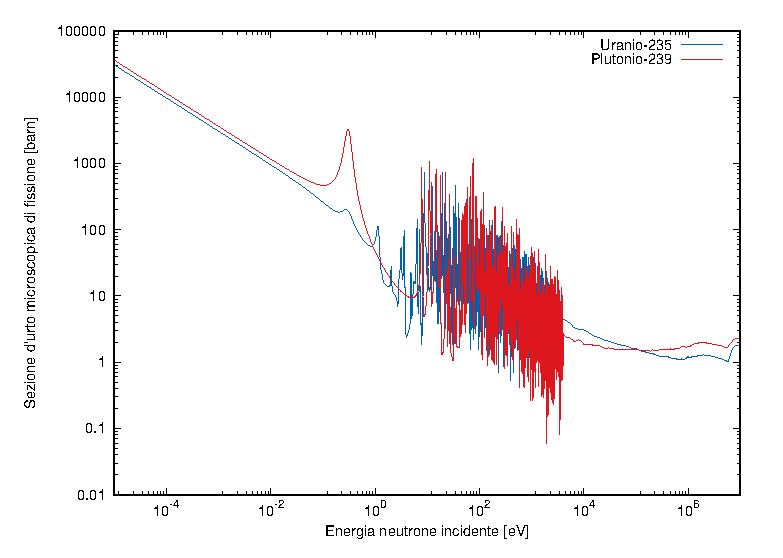
\includegraphics[width=0.7\textwidth]{./graph/sezurto}
\caption{Confronto sezioni d'urto microscopiche di fissione del $^{235}U$ e del 
$^{239}Pu$ della libreria JEFF.3.3.}\label{sezurto}
\end{figure}
%%%%%%%%%%%%%%%%%%%%%%%%%%%%%%%%%%%%%%%%%%%%%%%%%
La sezione d'urto macroscopica, a differenza della microscopica, si applica ad 
un specifico materiale, ed è legata alla sezione d'urto microscopica secondo la 
relazione
\begin{equation}
\Sigma_x (E) =\sum_{i=1}^I N_i \sigma_{x,i} (E)\,,
\end{equation} 
dove $N_i$ rappresenta la densità atomica del materiale considerato e $x$ il 
tipo di reazione considerato.
La densità di nuclei di un dato materiale può essere calcolata da
\begin{equation}
N_i=\frac{\rho_i A}{M_i} \,,
\end{equation}
dove $\rho$ è la densità del materiale (g/cm$^3$), $M$ è la massa atomica del 
singolo nuclide ($u$) e $A$ il numero di Avogadro definito come 6.022084$ \cdot$ 
10$^{23}$ (u/g).

Il tasso di reazione $R_x$ può essere definito attraverso il 
flusso neutronico integrato $\phi(\vec{r},E)$, ovvero la popolazione neutronica 
che attraversa il mezzo, secondo la relazione
\begin{equation}
\label{tasso_di_reazione}
R_x(E)=\Sigma_x(E) \phi(\vec{r},E) \,.
\end{equation}
Le principali reazioni nucleari possibili si possono catalogare in reazione di 
scattering, fissione e cattura radioattiva; le proprietà nucleari del mezzo 
considerato sono rappresentate dalla sezione d'urto macroscopica totale 
$\Sigma^T$, definita come la somma delle tre (per semplicità) sezioni d'urto 
macroscopiche quali la sezione d'urto macroscopica di scattering $\Sigma^S$, la 
sezione d'urto macroscopica di fissione $\Sigma^F$ e la sezione d'urto 
macroscopica di assorbimento $\Sigma^A$.
Pertanto le sezioni d'urto macroscopiche, oltre alla dipendenza dall'energia 
del 
neutrone, sono influenzate dalle proprietà termodinamiche dei nuclei che 
compongono il mezzo, ad esempio la temperatura e la densità. Infatti è noto il 
fenomeno dell'effetto Doppler, di particolare importanza nei reattori nucleari 
termici, che a seguito di un aumento di temperatura 
causa un appiattimento della risonanza nella zona risonante delle sezioni d'urto.

\subsection{Effetti di autoschermo e effetto Doppler}

%%%%%%%%%%%%%%%%%%%%%%%%%%%%%%%%%%%%%%%%%%%%%%%%%%%%%%%%%%%
\Figure[width=0.7\textwidth]{./figure/reactor/doppler.png}{Effetto 
Doppler.}{doppler}
\Figure[width=0.7\textwidth]{./figure/reactor/Doppler-Broadening-238U.png}{
Sezioni d'urto dell' $^{238}U$ con effetto Doppler.}{doppler1}
%%%%%%%%%%%%%%%%%%%%%%%%%%%%%%%%%%%%%%%%%%%%%%%%%%%%%%%%%%%
In molti casi la quantità di reazioni di assorbimento viene drammaticamente 
ridotta nonostante la sezione d'urto microscopica del materiale rimanga 
invariata. Questo fenomeno è comunemente conosciuto come \textit{risonanza di 
autoschermo} ed esso contribuisce alla stabilità del reattore. 
Sono conosciuti due tipi diversi di autoschermo: quello energetico e quello 
spaziale.

Nel primo caso, la vicinanza delle risonanze causa un aumento delle probabilità 
di assorbimento quando il neutrone possiede una energia prossima alle 
risonanze. 
Questo provoca una riduzione dell'effettivo assorbimento per nucleo dovuto alla 
depressione del flusso neutronico $\phi(E)$ vicino alla risonanza rispetto al 
flusso neutronico piano. 
Alle energie appena sotto la risonanza, dove $\sigma_a(E)$ diventa di nuovo 
piccola, il flusso neutronico raggiunge quasi lo stesso valore che possedeva 
prima della risonanza.

Mentre nel secondo caso, l'effetto di autoschermo spaziale è un fenomeno 
connesso principalmente con l'eterogeneità del nocciolo del reattore.
Infatti il rivestimento superficiale del combustibile scherma geometricamente 
gli strati interni dal flusso neutronico, portando un flusso neutronico 
relativamente più debole all'interno della barra di combustibile.
Infatti con l'aiuto dell'effetto di autoschermo spaziale i neutroni sono più 
facilmente assorbiti dai nuclei vicini alla superficie del combustibile, soprattutto per energie intermedie.

L'effetto di autoschermo spaziale e energetico causa un significativo aumento 
della probabilità di fuga dalla risonanza $p$, che ha luogo principalmente per 
reattori eterogenei rispetto a quelli omogenei.

In particolare l'effetto di autoschermo energetico è influenzato dalla 
temperatura del materiale ed è dovuto all'allargamento delle risonanze per 
effetto Doppler.
All'aumentare della temperatura, aumenta anche l'agitazione termica dei nuclei 
del materiale causando un allargamento delle risonanze dovuto all'effetto 
Doppler. 
Il flusso neutronico segue il comportamento del cambiamento della risonanza in 
maniera opposta, portando ad una riduzione dell'effetto di autoschermo e 
aumentando la sezione d'urto microscopica di assorbimento effettiva.

Questi fenomeni comportano una variazione negativa di reattività a seguito di un 
aumento di temperatura. In particolare se aumenta la temperatura del 
combustibile, l'effetto pronto dovuto a questi fenomeni, aumenta l'assorbimento 
dei neutroni provocando una diminuzione del flusso neutronico e quindi delle 
reazioni di fissioni che provocano una riduzione della potenza termica 
rilasciata dal reattore.
Infatti l'allargamento Doppler delle risonanze è un importante fenomeno che 
aumenta la stabilità del reattore ed è considerato come fattore dominante 
nei reattori termici nella valutazione del coefficiente di temperatura, 
definito in \eqref{coeff_di_temp}.
Infatti questo coefficiente è anche chiamato coefficiente pronto di temperatura 
perché causa una risposta immediata ad un cambio di temperatura e nella maggior 
parte dei reattori termici è negativo.

Nei reattori veloci, l'effetto Doppler diventa meno dominante, ma dipende 
fortemente dallo spettro neutronico e dal tipo della matrice di combustibile 
adottata. Nei reattori veloci, altri effetti, come l'espansione termica assiale 
delle pastiglie di combustibile o l'espansione radiale del nocciolo del 
reattore, possono contribuire allo stesso modo al coefficiente di temperatura.

\section{Reattori veloci}

\begin{figure}[!htb]
\centering
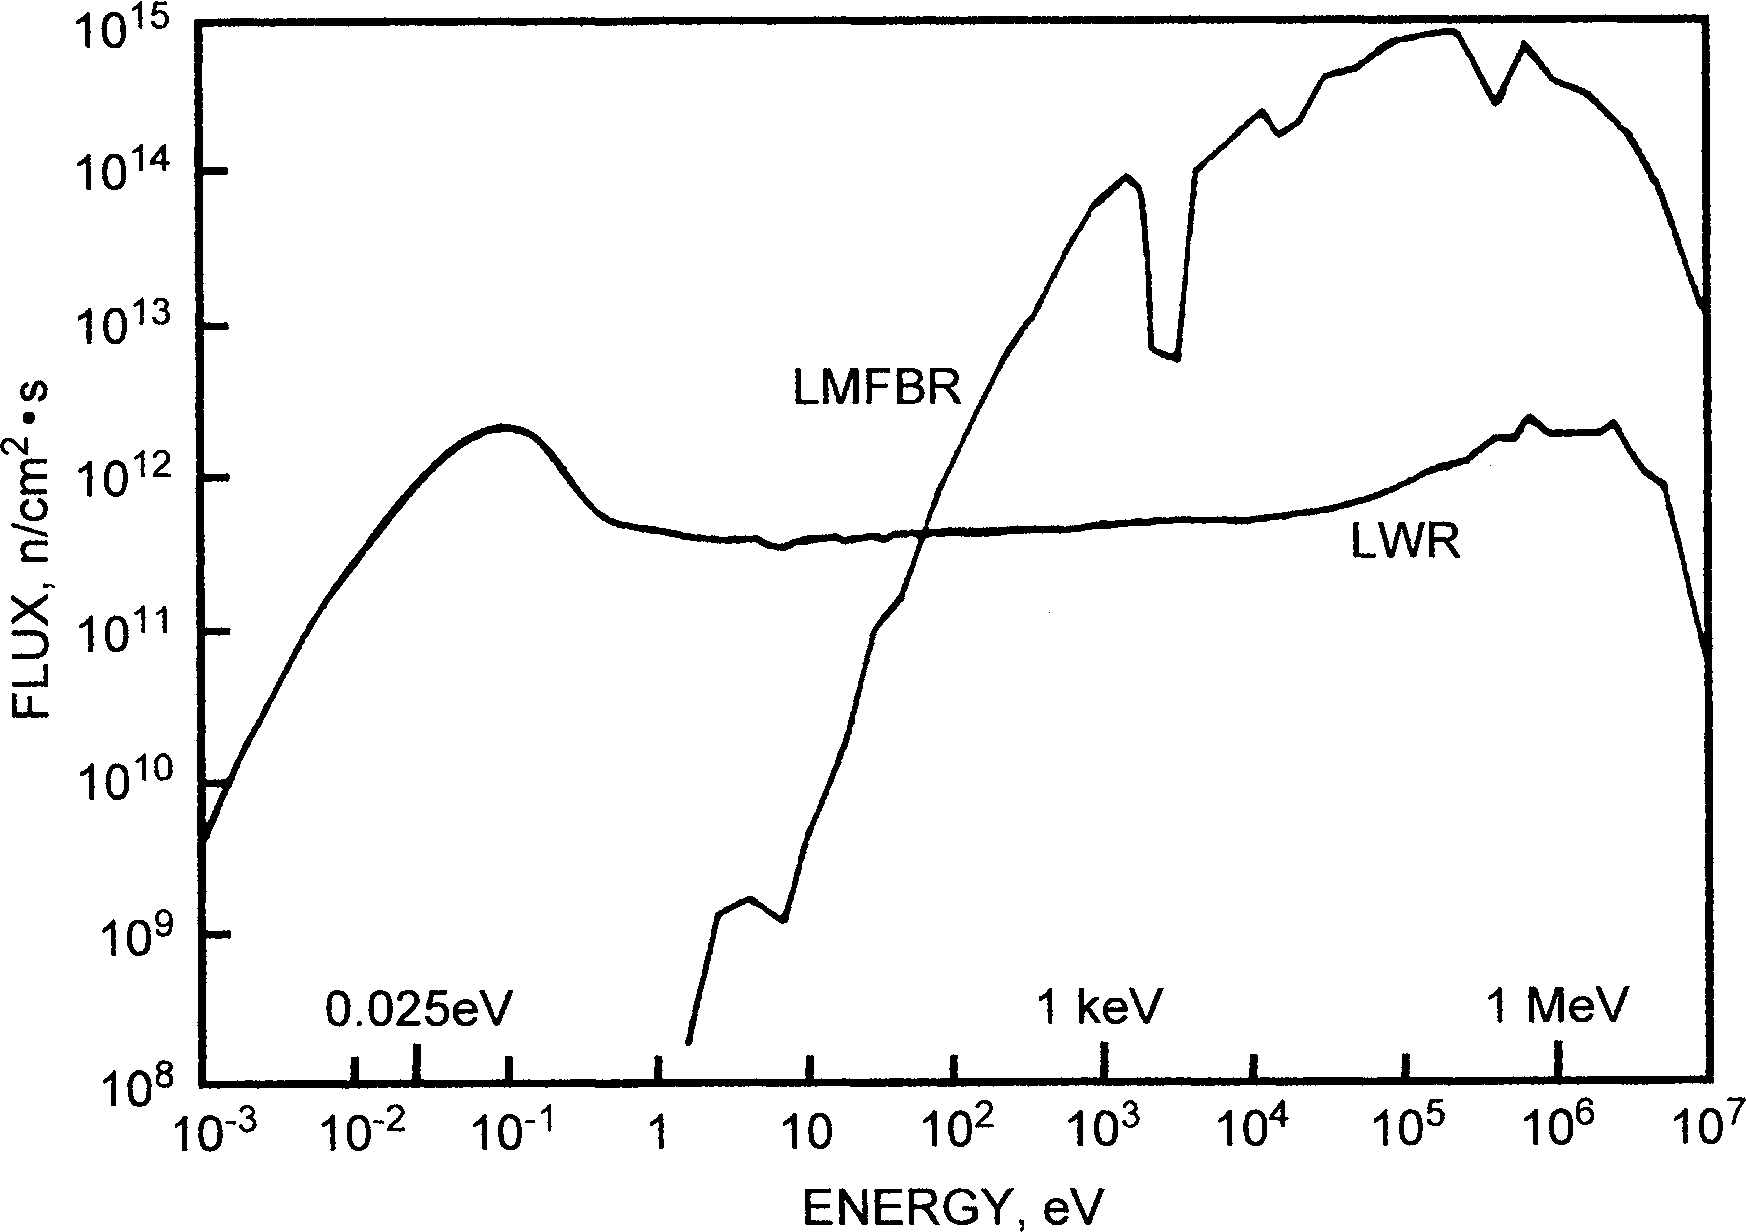
\includegraphics[width=0.7\textwidth]{./figure/reactor/energydistributionreactors.png}
\caption{Distribuzione dell'energia dei neutroni emessi in un evento di 
fissione.}\label{distribuzione_energetica_fissione}
\end{figure}

Si possono distinguere i reattori nucleari in termici o veloci, in base allo 
spettro neutronico utilizzato per indurre a fissione.
Nei reattori termici, essendo la probabilità più alta di indurre fissione alle 
energia termiche, i neutroni emessi dalla fissione che possiedono un'alta energia dovranno essere rallentati attraverso urti elastici finché il neutrone non 
diventa termico. 
Per rallentare i neutroni si utilizza un moderatore di neutroni, composto da 
atomi leggeri che permettono al neutrone incidente di perdere molta energia a 
seguito di collisioni.
I moderatori di neutroni più comuni, sia per la disponibilità che per 
l'economicità, sono ad acqua leggera $H_2O$ (LWR) e ad acqua pesante $D_2O$ (HWR). 
In questi tipi di reattori ad acqua leggera, si utilizza un combustibile 
generalmente poco arricchito (3-5$\%$), dove l'isotopo fissile generalmente 
$^{235}U$ è in piccola percentuale rispetto agli altri isotopi dell'uranio. 

In natura l'uranio naturale è composto dal 0.005$\%$ di $^{234}U$, 0.72$\%$ di 
$^{235}U$ e 99.275$\%$ di $^{238}U$. Quindi per essere utilizzato in impianti 
nucleari ad acqua leggera dovrà subire un processo di arricchimento, anche 
dovuto al fatto che l'acqua oltre ad essere un buon moderatore di neutroni e 
allo 
stesso tempo un buon assorbitore di neutroni, i quali se sono assorbiti sono 
rimossi dalla reazione a catena.
Nei reattori ad acqua pesante, invece, è possibile utilizzare combustibile poco 
arricchito o direttamente uranio naturale, in quanto l'acqua pesante è meno 
incline ad assorbire neutroni rispetto all'acqua leggera.
Nel tempo i reattori termici si sono sviluppati, e tuttora sono quelli 
maggiormente costruiti per la produzione di energia da fonte nucleare. Questi 
tipi di reattori, tuttavia possiedono problemi nello smaltimento del 
combustibile esausto, in cui a seguito delle reazioni a catena sono stati 
prodotti diversi isotopi radioattivi con un'emivita molto alta, come per 
esempio 
gli attinidi, i quali dovranno essere gestiti in modo opportuno.
Inoltre in questi reattori, l'acqua svolge anche la funzione di refrigerare gli 
elementi di combustibile, ovvero come vettore termico, e quindi asportare 
calore 
per la successiva generazione di vapore. Come in sistemi energetici 
convenzionali, il vapore prodotto viene immesso in turbine che attraverso 
l'accoppiamento ad un alternatore producono energia elettrica.
In molti reattori, la produzione di energia avviene in circuiti secondari 
evitando di mandare in turbina vapore attivato a seguito dell'assorbimento di 
neutroni nel nocciolo, così da semplificare l'eventuale smantellamento degli 
elementi che a loro volta si attiverebbero. 


I reattori veloci, a differenza dei reattori termici, utilizzano uno spettro di 
fissione veloce e di conseguenza le fissioni sono indotte da neutroni ad alte 
energie. 
Tuttavia affinché la reazione a catena si autosostenga attraverso neutroni veloci è 
necessario utilizzare un combustibile ad alto arricchimento, generalmente ad 
ossidi misti (MOX) con un contenuto di uranio-plutonio di circa 30$\%$. 
Uno dei vantaggi più importanti dei reattori veloci è l'alta efficienza di 
fertilizzazione. 
\subsection{Reattori autofertilizzanti}
Oltre agli isotopi fissili, esistono isotopi fissionabili e isotopi fertili. Gli 
isotopi fissionabili sono in grado di dar luogo a fissione con neutroni che 
possiedono sufficiente energia cinetica per superare una certa soglia di energia. Invece gli 
isotopi fertili sono isotopi che a seguito dell'assorbimento di un 
neutrone si trasmutano in isotopi fissili.
Un esempio di isotopo sia fissionabile che fertile è l'uranio $^{238}U$. 
Infatti dall'assorbimento di un neutrone si produce l'isotopo fissile $^{239}Pu$, , attraverso la seguente catena di decadimento 
\begin{equation}
\label{fertpu}
^{238}_{92}U + ^{1}_{0}n \, \longrightarrow ^{239}_{92}U  \xrightarrow{\beta^-}
 \, ^{239}_{93}Np  \xrightarrow{\beta^-} \, ^{239}_{94}Pu\,.
\end{equation}
Un altro esempio di isotopo fertile, è il torio $^{232}Th$ che sempre 
attraverso l'assorbimento di un neutrone subisce la trasformazione seguente
\begin{equation}
\label{fertth}
^{232}_{90}Th + ^{1}_{0}n \, \longrightarrow ^{233}_{90}U  \xrightarrow{\beta^-}
 \, ^{233}_{91}Pa  \xrightarrow{\beta^-} \, ^{233}_{92}U\,,
\end{equation}
La possibilità di produrre isotopi fissili dalla fertilizzazione di altri 
isotopi come appunto il torio $^{232}Th$ e l'uranio $^{238}U$, ha aperto la strada 
alla progettazione di reattori autofertilizzanti capaci di produrre più 
combustibile di quanto essi consumano (Breeder Reactor).
Oltre ai TBR (Thermal Breeder Reactor), sono molto interessanti dal punto di 
vista tecnologico FBR (Fast Breeder Reactor).

Rispetto alle energie
termiche, alle energie veloci è più probabile che avvenga l'assorbimento del neutrone da parte di isotopi fertili, 
così da creare un ciclo chiuso di combustibile dovuta alla trasmutazioni in isotopi fissili.
Inoltre il reattore operando in campo veloce non necessita più della presenza 
di un moderatore di neutroni, in quanto è indispensabile non rallentare i neutroni 
attraverso collisioni per portarli alle energie termiche.
Un altro vantaggio dovuto all'assenza del moderatore è di permettere la costruzione di 
reattori più compatti e pertanto questa tecnologia ha permesso il suo utilizzo come propulsori in ambito 
navale e spaziale.
Ci sono differenti tipi di reattori veloci e uno dei migliori sviluppi 
consiste 
nel reattore autofertilizzante veloce raffreddato ai metalli liquidi (Liquid 
Metal Fast Breeder Reactor - LMFBR).
In questo caso si utilizza come vettore termico un metallo liquido, che ha 
ottime proprietà termodinamiche di trasferimento del calore e allo stesso tempo 
risulta un pessimo moderatore di neutroni grazie al suo elevato peso atomico.
In questa categoria rientrano gli SFR (Sodium Fast Reactor) che utilizzano come 
refrigerante il sodio liquido e gli LFR (Lead Fast Reactor) che utilizzano 
invece il piombo liquido.

\subsection{Rateo di conversione}
Un importante fattore nei reattori autofertilizzanti è il rateo di conversione 
del 
materiale fertile in fissile.
Pertanto lo spettro neutronico veloce, comparato a quello termico, è molto più 
efficiente nel distruggere attinidi a causa del rateo maggiore di reazione di cattura.
In questo contesto, gli elementi transuranici possono essere rimossi dal 
combustibile nucleare utilizzato e successivamente trasmutati in elementi con 
una vita più breve in reattore veloci dove nel frattempo producono energia.
La trasmutazione degli elementi transuranici riduce il peso ambientale a lungo 
termine dell'energia nucleare attraverso una significante riduzione della dose 
rilasciata e della radiotossicità.
La fertilizzazione del combustibile nucleare è ottenuta da due processi di 
conversione nucleare dove il nucleo fissile è prodotto attraverso una cattura 
neutronica in nuclei fertili descritti dell'equazioni \eqref{fertpu} e 
\eqref{fertth}.

Il processo di conversione è descritto quantitativamente  dal termine di 
rateo di conversione $C$, il quale è definito come il rapporto tra il numero medio 
di nuclei fissili prodotti e il numero di nuclidi consumati.
Quando il termine $C$ risulta essere >1 , si definisce come rateo di 
fertilizzazione, in quanto viene prodotto più fissile di quello che viene 
consumato.
La capacità fertilizzante di un reattore può essere stimata attraverso un 
bilancio di neutroni 
\begin{equation}
 L + A_{fissile}+A_{fertile}+A_{altri}=\nu F_{fissile} + \nu F_{fertile} \,,
\end{equation}
dove $L$ è il rateo dei neutroni persi per via delle fughe, $A$ il rateo dei neutroni 
assorbiti dal relativo materiale mentre $\nu F$ rappresenta il rateo di 
produzione dei neutroni dovuti alla fissione.
Normalizzando l'equazione con $A_{fissile}$ e sistemando si ottiene l'equazione
\begin{equation}
 C=\frac{A_{fertile}}{A_{fissile}}=(\eta-1)+\varepsilon - (l_A + l_L + l_D) \,,
\end{equation}
dove $\eta$ è il numero di neutroni prodotti dalla fissione dell'isotopo 
fissile, $\varepsilon$ il numero di neutroni prodotti dalla fissione 
veloce nell'isotopo fertile, $l_A$ il numero di neutroni persi a seguito di 
assorbimento in altri materiali e $l_L$ è il numero di neutroni persi a seguito 
di fughe. Inoltre è stato aggiunto il termine $l_D$ che rappresenta la scomparsa 
di isotopo fissile per trasmutazione, come per esempio 
del plutonio $Pu$ in americio $Am$.
Il fattore di fertilizzazione $\eta(E)$ gioca un ruolo importante nel 
determinare il rateo di conversione o di fertilizzazione. Esso rappresenta il 
numero medio di neutroni emessi per evento di fissione per ogni neutrone 
assorbito dal combustibile fissile.

\Figure[scale=0.8]{./graph/nubar}{Numero totale di neutroni prodotti per evento 
di fissione dei principali isotopi fissili.}{NE}

Dalla Figura \ref{NE} si nota che il numero di neutroni prodotti, sia pronti 
che 
ritardati, è maggiore per l'isotopo $^{239}Pu$ rispetto agli altri isotopi 
fissili e che per energie maggiori a circa 100keV, il numero di neutroni emessi 
per evento di fissione aumenta rapidamente con l'aumentare dell'energia.
La capacità di fertilizzazione di un reattore è rappresentata dal tempo in 
cui la quantità di fissile raddoppia. 
Inoltre uno spettro veloce consente di ottenere un maggiore contributo di 
fissione veloce $\varepsilon$ del fertile, in quanto la fissione del fertile come il 
$^{238}U$ (fissionabile) è possibile solo se il neutrone incidente possiede 
energia sopra una certa soglia.
Il fattore di fissione veloce $\varepsilon$ rappresenta il rapporto tra la 
quantità dei neutroni prodotti dalla fissione veloce dall'isotopo fertile 
rispetto a quelli assorbiti dall'isotopo fissile.

In definitiva il rapporto di fertilizzazione aumenta se si mantiene uno spettro 
neutronico veloce e quest'ultimo è controllato dalla densità degli atomi 
pesanti contenuti nel refrigerante e negli elementi strutturali. \cite{yang}

\section{Reattori veloci raffreddati a piombo}

\begin{figure}
\centering
  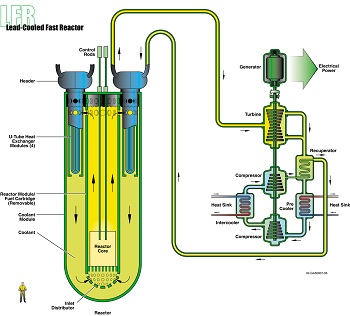
\includegraphics[width=0.7\textwidth]{./figure/reactor/lfr.jpg}
\caption{Schema d'impianto del reattore veloce
refrigerato a piombo.}
\end{figure}

I reattori veloci raffreddati a piombo liquido sono caratterizzati da uno spettro 
neutronico veloce e sono refrigerati con metallo liquido quale il piombo o, in 
alcuni casi, con una lega eutettica di piombo-bismuto, entrambi operanti a bassa 
pressione e con alte temperature operative.
La scelta del sistema di raffreddamento a piombo presenta numerosi vantaggi 
applicati ai sistemi nucleari.
Alcune caratteristiche dei metalli liquidi sono 
presentate nella Tabella \ref{pb}.
Infatti il piombo risulta essere un liquido denso, quando è mantenuto sopra la 
normale temperatura di fusione, con ottime proprietà termodinamiche mentre le 
sue proprietà nucleari, come la bassa tendenza di assorbire o rallentare 
neutroni, garantisce il sostentamento di uno spettro veloce di neutroni 
richiesto dai reattori veloci.

In termini di sicurezza, un importante vantaggio è l'alta temperatura di 
ebollizione del piombo che permette di eliminare eventuali problemi di 
ebollizione del refrigerante e garantisce così una semplificazione di progetto 
e 
un aumento dell'economicità delle prestazioni.
Inoltre essendo un reattore che opera a pressione atmosferica, un eventuale 
incidente di perdita di refrigerante (LOCA) può essere evitato progettato un'appropriata
struttura del recipiente (vessel). Questo offre in aggiunta 
potenziali semplificazioni di impianto in quanto non è necessario il complesso 
processo di gestione simultanea della temperatura, pressione e livello di 
refrigerante (come nei reattori refrigerati ad acqua).

Un altro vantaggio offerto dall'utilizzo del piombo come refrigerante, 
comparato 
specialmente ad acqua e sodio, è la bassa 
reattività chimica con aria
evitando così reazioni violente ed esotermiche.
Oltre ad essere un materiale relativamente inerte, si aggiunge anche l'elevata 
capacità di schermare radiazioni e trattenere prodotti di 
fissione e/o altri materiali che possono essere rilasciati dal combustibile in 
eventi incidentali. Questo consente l'eliminazione della necessità di avere un 
sistema di raffreddamento intermedio per isolare il refrigerante primario 
dall'acqua e il vapore, necessari per i sistemi di conversione dell'energia.
In caso di fuoriuscita accidentale di refrigerante, il piombo solidificherebbe 
abbastanza velocemente, senza che ci siano perdite non controllate, garantendo 
così una sicurezza passiva a questo tipo di incidenti.

Tuttavia ci sono alcune problematiche relative all'uso del piombo che sono in 
fase di valutazione, quali l'alta temperatura di 
fusione, 
la sua opacità, il rischio sismologico e soprattutto la potenziale corrosione 
a 
contatto con elementi strutturali in acciaio. 
\begin{table}[!htb]
 \centering
\begin{tabular}{lccc}
\toprule
 & Piombo & LBE & Sodio \\
\midrule
 Simbolo & $^{207}Pb$ & $^{207}Pb-^{209}Bi$ & $^{23}Na$ \\

 T fusione & 327.5$^\circ$C & 125$^\circ$C & 98$^\circ$C\\
  %\rowcolor{mygray}
 T ebollizione & 1749$^\circ$C &  1670$^\circ$C &882.8$^\circ$C\\
 Reattività  & Inerte & Inerte & Altamente  \\
 con acqua e aria & & & reattivo \\
\bottomrule
\end{tabular}
\caption{Confronto proprietà dei materiali utilizzati come possibili 
refrigeranti in reattori veloci a metalli liquidi. \label{pb}}
\end{table}

L'alta temperatura di fusione del piombo richiede che il sistema primario di 
raffreddamento sia mantenuto ad una temperatura tale da prevenire la 
solidificazione o almeno da garantire una adeguata circolazione del 
refrigerante 
a livello del nocciolo.
In questo contesto, la lega eutettica di piombo-bismuto (LBE) garantisce una 
minore temperatura di fusione rispetto a piombo puro, oltre a migliori 
proprietà 
termodinamiche. Tuttavia questa lega presenta svantaggi legati all'attivazione 
neutronica del bismuto attraverso la trasformazione
\begin{equation}
^{209}_{83}Bi + ^{1}_{0}n \, \longrightarrow ^{210}_{83}Bi  \xrightarrow{\beta^- 
; \text{5 giorni}} \, ^{210}_{84}Po  \,.
\end{equation}
Il polonio-210 risulta essere un potente emettitore di radiazioni alfa e produce 
un significativo aumento di calore nel refrigerante stesso.
Inoltre il bismuto è un elemento poco disponibile in natura e quindi molto 
costoso rispetto al semplice piombo che risulta essere abbondante e facilmente 
reperibile.

L'opacità del piombo presenta problematiche relative all'ispezione e al 
monitoraggio delle componenti interne al nocciolo e la sua alta massa atomica 
rende necessarie attente considerazioni al fine di prevenire impatti sismici.
Una delle sfide più importanti da risolvere, è la tendenza ad essere 
altamente corrosivo nei confronti di componenti in acciaio, accelerata dalle 
alte temperatura. Per questo motivo è necessario uno sviluppo in materiali 
strutturali capaci di resistere alla corrosione del piombo alle alte 
temperature.

In definitiva, questi tipi di reattori possono avere molte applicazioni, tra 
cui 
la produzione di energia elettrica, produzione di idrogeno e processi di 
riscaldamento.
La loro caratteristica di sostenere una catena di fissione veloce, come per gli 
altri reattori veloci, permette un'eccellente gestione delle risorse 
utilizzando 
un ciclo chiuso di combustibile attraverso un'efficiente conversione 
dell'uranio 
fertile. Possono anche essere utilizzati come bruciatori al fine di consumare 
attinidi in combustibili esausti proveniente da reattori LWR (Light Water 
Reactor).
La sicurezza passiva, offerta dalla scelta del piombo come refrigerante, 
permette una semplificazione dei sistemi di sicurezza e una maggiore 
affidabilità del reattore stesso.

Numerosi reattori di questo tipo sono in via di sviluppo in differenti paesi 
che 
includono Cina, Russia, USA, Svezia, Corea e Giappone.
%\cite{overview}
I concetti dei sistemi nucleari raffreddati a piombo rappresentati dalla 
``Generation IV International Foum (GIF) e System Research Plan (SRP)" sono 
basati sul sistema europeo dei sistemi raffreddati a piombo ELFR (in Figura 
\ref{elfr}), su quello russo BREST-OD-300 (in Figura \ref{brest}) e su
quello americano SSTAR (in Figura \ref{sstar}).
\Figure[scale=0.6]{./figure/reactor/elfr.png}{Schematico rappresentativo del 
reattore ELFR.}{elfr}
\Figure[scale=0.6]{./figure/reactor/brest.png}{Modello rappresentativo del 
reattore BREST-OD-300.}{brest}
\Figure[scale=0.6]{./figure/reactor/sstar.png}{Modello rappresentativo del 
reattore SSTAR.}{sstar}

Infatti a livello internazionale, il GIF ha identificato nella tecnologia LFR un gran 
potenziale per soddisfare gli obiettivi stabili per la nuova generazione di 
impianti nucleari di potenza.
In questo contesto ha considerato il progetto americano SSTAR, un piccolo 
sistema trasportabile di piccola taglia (10 - 100MWe), il progetto russo 
BREST-OD-300, un sistema di taglia intermedia, e infine il progetto europeo 
ELFR, un sistema più grande incentrato sulla generazione di energia elettrica 
(600MWe). In Tabella \ref{Starelsy} sono presenti le principale caratteristiche 
dei progetti appena citati.

Un importante passaggio nello sviluppo di reattori LFR in Europa è iniziato nel 
2006, quando EURATOM ha deciso di fondare il progetto ELSY (European Lead 
cooled 
SYstem) coordinato dall' Ansaldo Nucleare, sviluppando un innovativo progetto 
preconcettuale di un impianto industriale per la produzione di energia elettrica 
in grado di offrire un ciclo chiuso di combustibile \cite{cinotti2008elsy}.
Successivamente lo sviluppo degl LFR è continuato con il progetto LEADER 
(Lead-cooled European Advanced DEmonstration Reactor) iniziato nell'aprile 
2010, 
con lo scopo di sviluppare a livello concettuale un reattore critico di 
dimensioni industriali ELFR e, contemporaneamente, a livello dimostrativo la 
tecnologia LFR di piccola taglia (120MWe) presentato come ALFRED (Advanced 
Lead 
Fast Reactor European Demonstrator).
Al fine di sviluppare il progetto ALFRED, nel 2013 è stato istituito il 
consorzio FALCON (Fostering ALfred CONstruction), a cui partecipano Ansaldo 
Nucleare, ENEA e RATEN-ICN. La Romania ha espresso l'interesse di ospitare e 
supportare l'implementazione di ALFRED.
%%%%%%%%%%%%%%%%%%%%%%%%%%%%%%%%%%%%%%%%%%%%%%%%%%%%%%%%%%%%%%%%%%55
\begin{table}[!htb]
\centering
\small
\begin{tabular}{l c c c}
\toprule
Parametri & SSTAR & BREST-OD & ELSY \\
\midrule
Potenza termica & 45 MWth & 700 MWth & 1500 MWth \\
% \midrule
Potenza elettrica & 20 MWe & 300 MWe & 600 MWe \\ 
% \midrule
Rapporto di conversione & $\sim$1 & $\sim$1 & $\sim$1 \\
% \midrule
Efficienza termodinamica & 44$\%$& 43 - 44$\%$ & 42 $\%$ \\
% \midrule
Refrigerante primario & Piombo & Piombo & Piombo \\
% \midrule
Circolazione (a regime) & naturale & naturale & forzata \\
% \midrule
Circolazione (rimozione)  & naturale & naturale & naturale \\
% \midrule
Temperatura d'ingresso & 420$^\circ$C & 420$^\circ$C & 400$^\circ$C \\ 
nel nocciolo           &  &  \\
% \midrule
Temperatura d'uscita & \ 567$^\circ$C & 540$^\circ$C & 480$^\circ$C \\ 
dal nocciolo  &  &  &\\
% \midrule
% Tipologia di combustibile & MOX  & MOX & MOX\\
% \midrule
% Materiale del cladding & Acciaio  & Acciaio  \\
%                        & ferritico-martensitico &  $T91$\\
% \midrule
$T_{max}$ di resistenza termica & 650$^\circ$C & 650$^\circ$C & 550$^\circ$C\\ 
del cladding                    &  &  &\\
% \midrule
% Diametro del pin  & \mSI{25}{mm} & \mSI{10.5}{mm} \\
% del combustibile  &  &  \\
% \midrule
Dimensioni del nocciolo & 0.8 - 1.02m & 1.1 - 2.6m & 1.4 - 4.5m \\
(altezza -       &    &     \\
diametro  )   &    &     \\
% \midrule
Ciclo secondario & S-CO$_2$ & Vapore surriscaldato &  Vapore surriscaldato \\
\bottomrule
\end{tabular}
\caption{Caratteristiche principali dei reattori
LFR proposti dal GIF.}
\label{Starelsy}           
\end{table}
%%%%%%%%%%%%%%%%%%%%%%%%%%%%%%%%%%%%%%%%%%%%%%%%%%%%%%%%%%%%%555

\section{Advanced Lead Fast Reactor European Demonstrator}

Il progetto ALFRED si presenta con lo scopo di dimostrare le prestazioni 
ottenibili dalla tecnologia dei reattori veloci raffreddati a piombo, come 
punto 
di svolta per lo sviluppo della nuova generazione di sistemi energetici 
nucleari. Allo stesso tempo fornisce un ambiente sperimentale, accessibile a 
ingegneri 
e tecnici europei, per applicare ricerche e sviluppi in ambito nucleare, 
supportando innovazioni per la sicurezza e sostenibilità in futuri impianti di 
potenza relativa a questo tipo di tecnologia.

Gli obiettivi delle attività di progetto per ALFRED  si incentrano sul definire 
le principali caratteristiche e di progettare le linee guida per la costruzione 
dell'impianto ELFR. \cite{nurethalfred}
In aggiunta si deve accertare che i materiali sviluppati e adottati siano in 
grado 
di sostenere le alte temperature e di mantenere una caratterizzazione veloce 
del 
flusso.
Inoltre è richiesta la valutazione degli aspetti di sicurezza del reattore e 
la minimizzazione del costo complessivo dell'impianto.
L'obiettivo, riguardante la neutronica, è principalmente di investigare la 
fattibilità di un \textit{nocciolo adiabatico}, il quale è un problema cruciale 
per 
l'attuale sostenibilità nei confronti delle risorse naturali e dell'impatto 
ambientale. Il concetto di nocciolo adiabatico, così chiamato, si riferisce 
alla 
possibilità di ottenere un ciclo chiuso di combustibile al fine di ottimizzare 
le risorse naturali e di ridurre la produzione di attinidi, i quali 
potrebbero essere continuamente riciclati. \cite{adiabaticgrasso}

Data la potenza prevista, il reattore ALFRED appartiene alla categoria dei 
SMRs (Small Modular Reactors). 
Gli SMRs sono definiti come reattori di piccola taglia (minore di 300 MWe) in 
grado di essere installati come moduli per impianti di potenza. 
La loro potenzialità è racchiusa nella possibilità di essere costruiti in 
fabbriche controllate ed essere trasportarti ed essere disponibili per la 
produzione di calore o di energia, desalinizzazione di acqua o altri scopi 
industriali. 
Inoltre hanno caratteristiche di semplicità, sicurezza avanzata e richiedono 
risorse finanziare limitate, le quali possono essere molto attrattive per i 
paesi con poca esperienza in ambito nucleare. \cite{smrlocatelli}

Pertanto ALFRED e ELFR sono caratterizzati da potenze termiche differenti, e 
risulta ovvio che non tutti i parametri del nocciolo del reattore potranno 
essere mantenuti uguali. 
In particolare l'arricchimento del combustibile e il rapporto di conversione 
sono diversi nei due noccioli e dunque la chiusura del ciclo di combustibile 
non 
rappresenta un obiettivo primario per il nocciolo di ALFRED.
D'altra parte, i materiali considerati sono gli stessi eccetto per i materiali 
di rivestimento, in quanto è necessario un tempo per la qualificazione di 
rivestimenti avanzati non compatibile con i tempi di progetto di ALFRED \cite{lodi2018stress}.
La sezione successiva, descrive il funzionamento del reattore dimostrativo 
ALFRED. I dati progettuali sono da considerarsi indicativi, in quanto sono in 
continuo cambiamento. 

\subsection{Sistema primario}

\begin{figure}[!htb]
\centering
  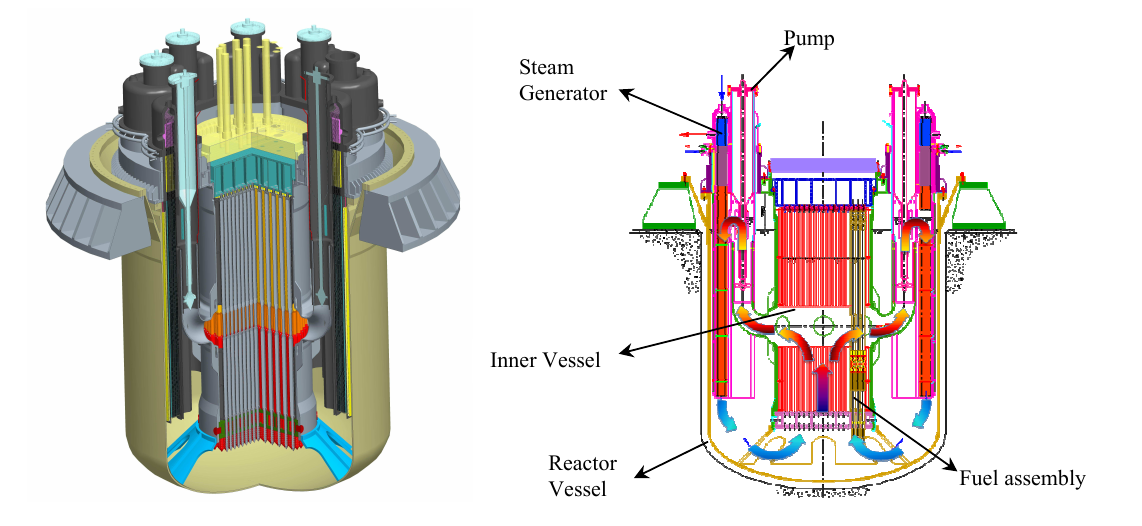
\includegraphics[width=0.7\textwidth]{./figure/reactor/alfred.png}
\caption{Schema 3D e sezione verticale relativi al reattore dimostrativo ALFRED.}\label{schemaalfred}
\end{figure}

\begin{table}[!htb]
\centering
\small
 \begin{tabular}{lcc}
\toprule
Parametro & Unità & Valore \\
\midrule
Potenza termica & MW  & 300 \\
Altezza totale del vessel & mm & 3500 \\
Raggio interno/esterno Inner vessel  & mm & 1475/1525 \\ 
Geometria della barra di combustibile & - & Esagonale incapsulata\\
Tipo di combustibile & - & MOX \\
Massima temperatura del combustibile & $^\circ$C & $\approx$2000\\
Picco di burn-up & MWd/kg & 100 \\
Materiale di rivestimento (cladding) & - & 15-15 Ti \\
Massima temperatura del rivestimento  & $^\circ$C & 550 \\
alle condizioni nominali & & \\
Massima temperatura del rivestimento& $^\circ$C & 750 \\
 durante ULOF & & \\
Refrigerante & - & Piombo fuso \\
Temperatura di ingresso refrigerante & $^\circ$C & 400 \\
Temperatura di ingresso refrigerante & $^\circ$C & 520 \\
Velocità media refrigerante & m/s & 1.28 \\
Velocità massima refrigerante & m/s & 2.00 \\
\bottomrule
\end{tabular}
\caption{Parametri principali che caratterizzano il reattore ALFRED 
\cite{alfredgrasso}.}
\end{table}

La configurazione del sistema primario è progettata a vasca (pool-type); questo 
concetto permette di contenere tutto il refrigerante primario all'interno del 
recipiente del reattore (vessel), eliminando così tutti i problemi relativi 
alla 
circolazione del liquido primario al di fuori di esso.
Le assembly del reattore presentano un semplice percorso per il flusso di 
refrigerante primario, composto da un flusso ascendente e discendente. La 
sorgente di calore, nel nocciolo, è localizzata nel flusso ascendente e gli 
scambiatori di calore (e generatori di vapore) sono situati nella parte alta del flusso 
discendente consentendo una efficiente circolazione naturale di refrigerante \cite{ponciroli2014object}. 
% Il refrigerante primario circola verso l'alto attraverso la pompa girante in senso 
% verticale, poi entra nei generatori di vapore attraverso il punto di entrata 
% del 
% piombo ed esce dai generatori di vapore.

Il reattore è costituito strutturalmente da diversi sistemi di contenimento, 
denominati vessel; in particolare il reactor vessel (RV) racchiude il reattore 
complessivo il quale è ricoperto da un safety vessel (SV), e all'interno è 
presente un altra suddivisione data dall'inner vessel (IN) che contiene il 
nocciolo.
Il reactor vessel ha una forma cilindrica con la parte inferiore tondeggiante 
come da Figura \ref{schemaalfred} e contiene il sistema primario di raffreddamento, l'inner vessel 
e quindi il nocciolo del reattore, gli scambiatori di calore per la successiva 
generazione di vapore e i sistemi di sicurezza.
Il safety vessel è costituito da uno strato di acciaio che ricopre la 
superficie 
del reactor vessel e ha una funzione di mitigare le conseguenze relative a 
perdite di piombo dovute a rotture accidentali. Il SV e RV sono distanziati 
sufficientemente da garantire ispezioni durante il servizio e sono sistemati in 
maniera tale che in caso di perdita il refrigerante primario rimasto sia 
sempre in grado di ricoprire l'entrata al generatore di vapore e il flusso 
percorso dal piombo rimanga invariato \cite{damiani2013conceptual}.
L'inner vessel possiede una forma cilindrica a doppia parete; la sua funzione 
principale di sostegno delle assembly di combustibile e di separazione tra 
plenum superiore caldo e quello inferiore freddo. Il flusso di piombo è guidato 
dall'uscita delle FA verso l'ingresso della pompa primaria attraverso un 
anello toroidale.

\subsection{Nocciolo del reattore}
\begin{figure}[!htb]
\centering
  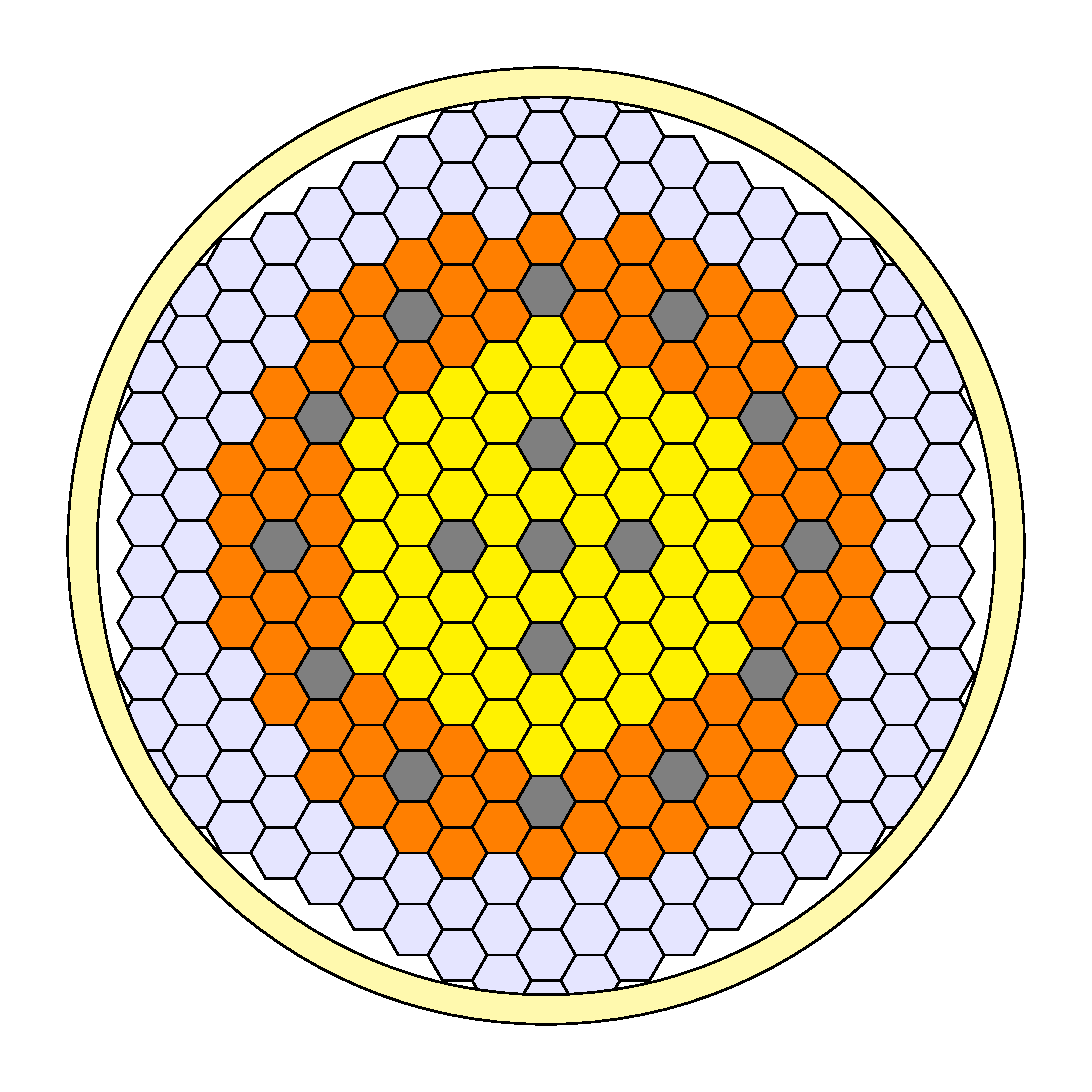
\includegraphics[width=0.7\textwidth]{figure/itex/skematic}
  \caption{Configurazione del nocciolo di ALFRED.}\label{distribuzione_nocciolo}
\end{figure}

Le assembly di combustibile sono sostenute inferiormente da una griglia, con 
una struttura scatolare che permette l'alloggiamento di esse e superiormente da 
un'altra griglia più rigida che invece svolge la funzione di inserimento delle 
assembly di combustibile durante le operazioni di reattore.
Sono presenti due sistemi diversi e ridondanti per le operazioni sul controllo 
di reattività, quali le barre di controllo (control rods) e barre di sicurezze 
(safety rods).
La configurazione del nocciolo è come quella mostrata in Figura 
\ref{distribuzione_nocciolo}, in cui sono presenti le assembly di 
combustibile 
con diverso 
arricchimento per la zona interna e quella esterna e i sistemi di controllo 
della reattività, quali le barre di controllo (control rods) e barre di 
sicurezze (safety rods).
Sono presenti infatti nella zona interna 56 assembly di combustibile (FA) e 78 
in 
quella esterna con un totale di 134, che si differenziano dall'arricchimento 
del combustibile definito in percentuale come il rapporto
\begin{equation}
\frac{Pu+^{241}Am}{Pu+^{241}Am+U}.
\end{equation}
Le barre di combustibile sono raggruppate in 126 costituendo così l'assembly 
complessivo (Fuel Assembly, FA), come in Figura \ref{FA}. I principali 
parametri 
progettuali sono definiti nella Tabella \ref{FAtable}.
\begin{figure}[!htb]
\centering
  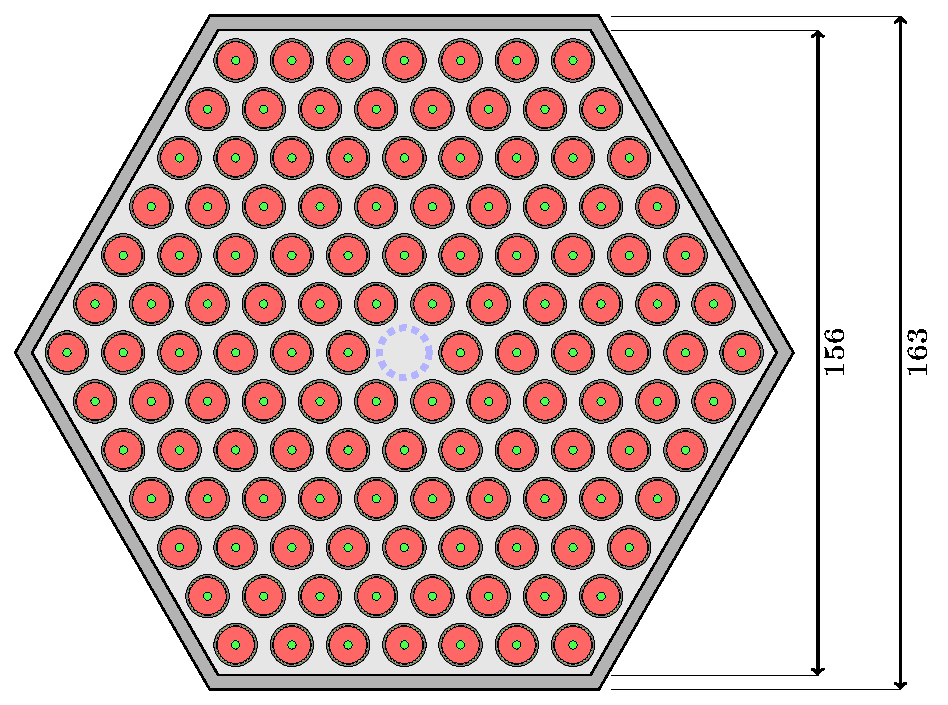
\includegraphics[scale=0.4,width=0.6\textwidth]{figure/itex/fullassembly_wq}
  \caption{Configurazione dell'assembly di combustibile di ALFRED.}\label{FA}
\end{figure}
\begin{table}[!htb]
\small
\centering
 \begin{tabular}{lcc}
\toprule
Parametro & Unità & Valore \\
\midrule
Numero totale di assembly di combustibile (FA) & - & 134\\
FA interni e esterni & - &  56/78 \\
Barre di controllo  & - & 12 \\
Barre di sicurezza  & - & 4 \\
Sezione In-pile & - & 1 \\
Distanza tra i pins & mm & 13.86\\
Spessore involucro & mm & 4.0\\
Distanza tra gli involucri & mm & 5.0\\
Numero di pin per FA & - & 126\\
Diametro cavità pastiglia & mm & 2.0\\
Raggio della pastiglia & mm & 4.5\\ 
Spessore gap & mm & 0.15\\
Spessore del rivestimento & mm & 0.6\\
Diametro pin & mm & 10.5\\
Lunghezza plug inferiore & mm & 50\\
Altezza gas plenum & mm & 550\\
Altezza insulator inferiore  & mm & 10\\
Altezza attiva & mm & 600\\
ALtezza insulator superiore & mm & 10\\
Lunghezza spring & mm & 120\\
Lunghezza plug superiore & mm & 50\\
\bottomrule
\end{tabular}
\caption{Parametri dimensionali della barra di combustibile di ALFRED.}\label{FAtable}
\end{table}
Le assembly di combustibile, rappresentate interamente in Figura 
\ref{geometria_assembly}, sono progettate secondo una struttura chiusa ed 
esagonale al fine di contenere il combustibile disposto in pastiglie cave le 
quali costituiscono la regione attiva della barra e le zone dove è presente il 
gas di fissione.  
Le pastiglie di combustibile sono cilindriche e cave, progettate come in Figura 
\ref{pin}. Al centro della cavità della pastiglia è contenuto il gas di 
fissione, in particolare elio, il quale essendo inerte ha la funzione di 
isolante termico. Procedendo verso l'esterno è presente il combustibile 
racchiuso da una guaina (cladding) di un particolare acciaio, 15-15 Ti, con la 
funzione di rivestimento e protezione. E' presente uno spazio tra quest'ultimi 
in cui è contenuto il gas di fissione.

\begin{figure}[!htb]
\centering
  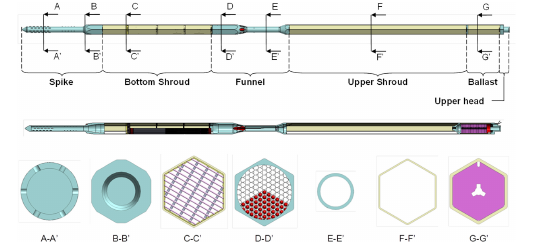
\includegraphics[width=0.7\textwidth]{figure/reactor/geomassembly.png}
  \caption{Rappresentazione una barra di combustibile di ALFRED 
\cite{alfredgrasso}.}\label{geometria_assembly}
\end{figure}
\begin{figure}
\centering
  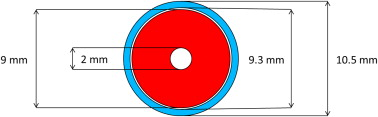
\includegraphics[width=0.7\textwidth]{figure/reactor/pinsection.png}
  \caption{Rappresentazione di una pastiglia di combustibile relativa alla 
barra 
di combustibile di ALFRED \cite{alfredgrasso}.}\label{pin}
\end{figure}
Per la composizione del combustibile è previsto l'utilizzo di un combustibile ossido misto (MOX), ovvero una 
miscela di ossido di uranio e ossido di plutonio $UO_2+PuO_2$, con 
arricchimento 
di $Pu$ del 20.5$\%$ per l'interno e del 26.2$\%$ per l'esterno.
Le percentuali isotopiche del plutonio e dell'uranio sono espresse in Tabella 
\ref{percentuali_isotopiche}. Il plutonio presenta un'alta percentuale di 
isotopo fissile $^{239}Pu$ mentre l'uranio è considerato come combustibile 
esausto proveniente da altri reattori convenzionali ed essendo praticamente 
tutto $^{238}U$ costituisce il materiale fertile che permette la chiusura del 
ciclo di combustibile.
\begin{table}[!htb]
\centering
 \begin{tabular}{cccc}
\toprule
Vettore plutonio & $\%$ atomi & Vettore uranio & $\%$ atomi \\
\midrule
$^{238}Pu$  &  2.348 & $^{234}U$  & 0.003 \\
$^{239}Pu$  & 57.015 & $^{235}U$  & 0.409 \\
$^{240}Pu$  & 26.951 & $^{236}U$  & 0.010 \\
$^{241}Pu$  & 6.069  & $^{238}U$  & 99.578 \\
$^{242}Pu$  & 7.616  &            &        \\
\bottomrule
\end{tabular}
\caption{Percentuale atomica dei vettori di plutonio e di uranio che compongono 
il combustibile MOX relativi al progetto ALFRED.}\label{percentuali_isotopiche}
\end{table}
La differente percentuale di arricchimento tra interno e esterno del nocciolo è 
realizzata per mantenere il flusso neutronico e quindi la potenza termica più 
uniforme lungo il profilo del reattore.
Le barre di controllo (CR) hanno il ruolo sia di normale controllo del 
reattore, 
come accensione, controllo di reattività e spegnimento) sia per SCRAM (arresto 
di emergenza) in caso di emergenze.
Le barre di sicurezza (SR) invece agiscono solamente in caso di SCRAM. 
L'estrazione avviene verso l'alto e l'inserzione verso il basso contro la forza 
di galleggiamento attraverso un sistema pneumatico. Nel caso in cui il sistema 
pneumatico sia non funzionante, la composizione in tungsteno forza una lenta 
inserzione per effetto della gravità. 
Per entrambi i sistemi, i materiali considerati sono $B_4C$ arricchito in 
$^{10}B$ che ha un'elevata sezione d'urto di assorbimento.

Il refrigerante primario è piombo fuso che presenta diversi vantaggi 
\cite{nurethalfred}. L'alta temperatura di ebollizione (1745 $^\circ$C) e la bassa 
pressione parziale consentono l'eliminazione di un pressurizzatore nel circuito 
primario a differenza dei reattori maggiormente in commercio quali i PWR 
(Pressure Water Reactor), semplificando la struttura dell'impianto. 
Essendo chimicamente inerte nei confronti di acqua e aria permette 
l'eliminazione di un circuito intermedio e l'installazione di unità di 
generazione del vapore all'interno del reactor vessel.
Le caratteristiche neutroniche relative al piombo di mantenere uno spettro 
neutronico veloce, consente di aver maggiore flessibilità sulla distanza tra le 
assembly di combustibile riducendo così le perdite di carico e aumentando così 
la circolazione naturale.
Tuttavia attraverso il progetto ALFRED, si dovranno affrontare la valutazione 
di 
alcuni aspetti critici dell'uso del piombo come refrigerante.
Infatti il piombo fuso interagisce con i materiali strutturali attraverso 
principalmente un meccanismo di corrosione e di erosione alle alte temperature.
Per tale motivo è previsto di operare in un intervallo di temperatura compreso 
tra i 400$^\circ$C e i 520$^\circ$C e un controllo sulla quantità di ossigeno dissolto 
nel piombo. 
La scelta di materiali adatti a resistere, come acciaio austenitico con basso 
contenuto di carbonio (AISI 316L), acciaio ferro-martensitico (T91) e acciaio 
15-15Ti, e l'utilizzo di rivestimenti superficiali, come l'alluminizzazione di 
superfici con Fe-Cr-Al-Y.
Infine per ridurre il processo di erosione, la velocità del flusso di piombo è 
limitata a circa 2-3m/s mentre per ridurre il rischio di solidificazione del 
piombo, è stato pensato un sistema attivo che mantiene il piombo fuso durante 
ogni normale operazione, per esempio durante spegnimenti pianificati.
Per ovviare al problema dell'opacità del piombo, ogni componente all'interno 
del 
reactor vessel è rimovibile e le assembly di combustibile si estendono oltre 
la superficie del piombo consentendo operazioni di rifornimento di combustibile 
senza l'utilizzo di strumentazioni particolari. 